\documentclass{sigchi}
\usepackage{balance}% to better equalize the last page
\usepackage{graphicx} % for EPS, load graphicx instead 
\usepackage{amsmath}
\usepackage[space]{grffile}
\usepackage[T1]{fontenc}
\usepackage{txfonts}
\usepackage{xspace}
\usepackage{mathptmx} % Comment if you want LaTeX's default font
%\usepackage[hyphens]{url} %allow breaking on - in URLs
\usepackage[breaklinks=true]{hyperref}
\usepackage{color}
\usepackage{booktabs}
\usepackage{textcomp}
\usepackage{microtype}% Improved Tracking and Kerning 
\usepackage{ccicons}
\usepackage[caption=false]{subfig}
%\usepackage{subcaption}
%\usepackage{caption} %for non-floating figures
\usepackage[nameinlink]{cleveref}
\usepackage[nocompress]{cite}%numerical order in citations
\usepackage{verbatim}%for \begin{comment}/\end{comment}
\usepackage[utf8]{inputenc}  %Allow symbols like °
\usepackage{cuted}
\usepackage{capt-of}
\usepackage{wrapfig}
\usepackage{float}
\usepackage[inline]{enumitem}

%For todo notes
\usepackage{todonotes}
\usepackage[multiple,para]{footmisc}

%Highlight todo; soul package has bugs so we do this instead
\usepackage[normalem]{ulem}
\newcommand\hl{\bgroup\markoverwith
  {\textcolor{yellow}{\rule[-.5ex]{.1pt}{2.5ex}}}\ULon}

\newcommand{\tv}[1]{\footnote{\href{https://thingiverse.com/thing:#1}{\footnotesize{\bf #1}}}\xspace}

\newcommand{\red}[1]{{\color{red}#1}}
\newcommand{\etal}{et~al.\@\xspace}
\newcommand{\bh}{Blowhole\xspace}
\newcommand{\at}{AirTouch\xspace}
\newcommand{\hhz}{Helmholtz\xspace}

%Comment out for camera-ready
\pagenumbering{arabic}

%Properly format cleverrefs
\crefname{figure}{Figure}{Figures}
\crefname{table}{Table}{Tables}
\crefname{equation}{Equation}{Equations}
%For referencing footnotes twice
\crefformat{footnote}{#2\footnotemark[#1]#3}
\creflabelformat{equation}{#2#1#3}

% Paper metadata (use plain text, for PDF inclusion and later
% re-using, if desired). Use \emtpyauthor when submitting for review
% so you remain anonymous.
\def\plainauthor{First Author, Second Author, Third Author}
\def\emptyauthor{}
\def\plainkeywords{Keywords}
\def\plaingeneralterms{General terms TBD, TBD}

% llt: Define a global style for URLs, rather than the default one
\makeatletter
\def\url@leostyle{%
\@ifundefined{selectfont}{
\def\UrlFont{\sf}
}{
\def\UrlFont{\small\bf\ttfamily}
}}
\makeatother
\urlstyle{leo}

% To make various LaTeX processors do the right thing with page size.
\def\pprw{8.5in}
\def\pprh{11in}
\special{papersize=\pprw,\pprh}
\setlength{\paperwidth}{\pprw}
\setlength{\paperheight}{\pprh}
\setlength{\pdfpagewidth}{\pprw}
\setlength{\pdfpageheight}{\pprh}

% Make sure hyperref comes last of your loaded packages, to give it a
% fighting chance of not being over-written, since its job is to
% redefine many LaTeX commands.
\definecolor{linkColor}{RGB}{6,125,233}

%\hypersetup{%
%	pdftitle={\plaintitle},
%	% Use \plainauthor for final version.
%	%pdfauthor={\plainauthor},
%	pdfauthor={\emptyauthor},
%	pdfkeywords={\plainkeywords}, 
%	bookmarksnumbered,
%	pdfstartview={FitH},
%	colorlinks,
%	citecolor=black,
%	filecolor=black,
%	linkcolor=black,
%	urlcolor=linkColor,
%	breaklinks=true,
%}

% create a shortcut to typeset table headings
\newcommand\tabhead[1]{\small\textbf{#1}}

\setlist{noitemsep}


\begin{document}
  \title{Enabling the Fabrication of Interactive 3D-printed Objects by
    Non-Experts and Novices}
  \author{%
    \alignauthor{Carlos E. Tejada\\
    \affaddr{Rochester Institute of Technology}\\
    \affaddr{Rochester, NY, US}\\
    \email{cet1318@rit.edu}}\\
  }

  \maketitle

  \begin{abstract}
    While digital fabrication has come great lengths since its inception
    decades ago, the promise of fabricating custom devices is still
    unfulfilled. Although the literature contains multiple efforts of adding
    interactivity to digitally fabricated objects, the techniques explored are
    often reserved for the more technically savvy, as they generally require
    extra knowledge from the maker. In this paper, we evaluate the current
    state-of-the-art in the fabrication of interactive objects, analyzing their
    inherent shortcomings. Inspired by the literature, we introduce an
    \itoolkit comprised of mechanisms to add interactivity to 3D-printed
    objects, in a maker-friendly way, and present our first steps in the
    population of this toolkit in the form of \bh, a system that allows the
    user to acoustically tag 3D-printed objects by embedding blowing-activated
    tags inside them.  We additionally discuss the current and future efforts
    towards enabling interactions in a maker-friendly way with the introduction
    of \at, a system that leverages airflow to enable touch interaction in
    digitally fabricated objects.
  \end{abstract}

  \section{Introduction}
    Although fabrication technology research may appear to be a recent trend in
    the Human-Computer Interaction (HCI) and computer graphics communities,
    this technology has been around for decades. The development of these
    technologies took place behind closed doors starting in the 1960s as a
    rapid prototyping technology. The expiration of major patents in 2009
    marked the beginning of the transition of this technology from the industry
    to the hands of the consumers, making these technologies accessible enough
    to be acquired by enthusiasts and hobbyists.

    This increased accessibility in digital fabrication equipment created a new
    category of fabricators. These fabricators (henceforth referred as makers)
    are interested in using these technologies to perform tasks of
    \emph{personal augmented fabrication}~\cite{Ashbrook:2016fga}: designing
    and fabricating objects that work with already existing ones, as Shewbridge
    \etal present in their study~\cite{Shewbridge:2014gl}.

    We believe that the next natural step in the evolution of these
    technologies is enabling its users to not only fabricate objects to
    interact with already existing ones, but to interact with the users
    themselves.This is corroborated by the numerous efforts published in the
    literature in the past years exploring novel ways to add interactivity to
    digitally fabricated objects (see Related Work for a literature review).

    However, previous work exploring the enabling of interactivity in digitally
    fabricated devices focus their efforts on the interactivity mechanisms
    themselves, without taking into consideration how the inclusion of these
    mechanisms adds more complexity to the fabrication process. The inclusion
    of electronic techniques, and advanced fabrication processes adds another
    level of complexity to the already complicated fabrication
    process~\cite{Hudson:2016hi, Mellis:2012ba, Weichel:2014ed} and can hinder
    the acceptance of these new technologies by novice users.

    Inspired by these limitations, in this paper we propose to enable
    interactions in digitally fabricated objects by utilizing naturally
    occurring properties (e.g. acoustic resonance, fluid dynamics). Rather than
    sensing the interactions of the user on the object itself, we propose to
    indirectly sense them by measuring the changes caused by the interaction to
    these properties using wearable sensing technologies. By externally sensing
    the effects the user's interactions have on these properties, the objects
    augmented with our mechanisms can be interacted with immediately after they
    finish printing, and do not require the addition of circuitry to enable
    interactions.

  \section{Research Questions}
    Based on the discussion presented above, we seek to answer the following
    research questions through our work:

    \begin{enumerate}
      \item What different natural properties can be leveraged to enable
        interactivity to digitally fabricated objects?
      \item How many different interaction mechanisms can we enable by making
        use of these properties?
      \item How does these interaction mechanisms perform against more complex
        mechanisms?
    \end{enumerate}

  \section{Related Work}
    Adding interactivity to 3D-printed objects has been a popular topic in the
    literature in recent years. While most efforts explore novel and
    interesting ways to make 3D printed objects more interactive, few
    concentrate their efforts in adding these interactive capabilities in an
    maker-friendly way---reserving this process for experienced and
    knowledgeable makers. Below we present a comprehensive survey of the
    different methods used to enable interactivity explored by the literature,
    categorized by the mechanisms used to enable them.

    \subsection{Acoustic}
      We can find in the literature multiple efforts leveraging acoustic
      properties to enable interactivity in printed objects.
      Stane~\cite{MurraySmith:2008ch}, for example, uses different surface
      textures that produce distinct acoustic signatures when rubbed with a
      finger. The sounds generated by these interactions are then captured by a
      microphone under the surface of the object and further analyzed and
      classified.

      An effort similar to Stane is Lamello~\cite{Savage:2015cs}.  Here, the
      authors leverage a series of components that, when interacted with,
      produce singular acoustic fingerprints by strumming fabricated comb-like
      structures that generates an identifiable signature. These tones are
      captured by contact microphones placed under the surface of the object,
      and identified using a classification pipeline. Notably, in this effort,
      the authors compiled a library of different interaction techniques that
      can be enabled using this mechanism, comprised of different types of
      buttons, sliders and dials.

      Efforts like Acoustruments~\cite{Laput:2015hn} enable more elaborate
      interactions by leveraging more elaborate fabrication processes. Here,
      the authors create acoustic pathways to route the audio emitted from a
      smartphone's speaker to its microphone, making use of physical controls
      to modify the signal going through this path. These controls can enable
      an vast number of interactions, from tilt to pressure sensing, and can be
      leveraged to create numerous application.

      Although these efforts enable an abundance of interesting interaction
      possibilities, they do it at the expense of complex fabrication
      techniques, often requiring multi-material printing techniques or
      post-print assemblies. While digital fabrication technologies are
      becoming ubiquitous, most novice makers are not experienced in complex
      fabrication techniques, limiting the reach of the interactions presented
      above.

    \subsection{Electric}
      While the use of electronic components to add interactivity to objects
      has been thoroughly used in manufacturing processes for decades, the
      advances in commercially available printers enable makers to fabricate
      their objects using a combination of conductive and nonconductive
      materials to enable new interaction modalities to their objects.

      An example of the efforts carried out leveraging electronic mechanisms to
      enable interactions is Steel-Sense~\cite{Vasilevitsky:2016hy}. In this
      effort, the authors leverage dielectric materials between two surfaces to
      create a hinge between two conductive surfaces, effectively sensing the
      angle of rotation of said surfaces.

      In Liquido~\cite{Schmitz:2016cv}, the authors leverage capacitive sensing
      and dielectric liquids (such as water) to augment the printed object with
      tilt and motion sensing. Using a dual extrusion printing process, the
      authors add conductive filament to the walls of a cavity, where the fluid
      is to be poured into. This cavity is then closed, and, when the liquid
      comes in contact with a sensor, capacitance increases.  These changes in
      the position of the liquid inside the object can be then translated to
      movement and orientation.

      The authors of PyzoFlex~\cite{Rendl:2012er} created a proprietary,
      printable, ferroelectric material, that, relying on the piezoelectric
      effect~\cite{Cady:1964fh}, can be used to add touch, pressure and bend
      sensing capabilities to 2D surfaces. This material also has pyroelectric
      characteristics, allowing it to sense changes in temperature in the
      printed object.

      Even though these new interaction capabilities enabled by the
      aforementioned efforts can unlock a wide variety of applications, they
      all require the user to possess certain electronic knowledge to fabricate
      these augmented objects. Not every maker has an electronic background,
      therefore these mechanisms are limited to a selected few.

    \subsection{Optic}
      Other researchers have explored enhancing printed objects using optical
      mechanisms. Notable efforts include Printed Optics~\cite{Willis:2012bc}
      by Willis \etal, where the authors are able to sense user input using
      light pipes and custom optical sensors. In this paper, the authors
      present different examples of augmented objects using this technology,
      like sliders, touch pads, and buttons.

      Another interesting effort is Sauron~\cite{Savage:2013kua}, where the
      authors make use of a camera, with an accompanying light ring, embedded
      to the inside of the printed object to detect the movements of areas of
      interest. This setup is augmented using a system of mirrors to allow the
      camera to  ``see'' around corners and bocks inside the object. This
      mechanism enabled a variety of interaction methods, like buttons,
      sliders, scroll wheels, etc.

      While both of the aforementioned efforts make use of optic mechanisms to
      enable very different interactions, they do so by increasing the
      complexity of the fabrication pipeline. In~\cite{Savage:2013kua} the
      maker is required to assemble the interactive components on the printed
      shell, as well as cameras and mirrors to sense the interactions, while
      in~\cite{Willis:2012bc} requires the use of intricate and expensive
      fabrication equipment and materials.

    \subsection{Metamaterial}
      3D-printing technologies enable the production of new types of
      metamaterials, since the properties of the material can be specified
      throughout different sections of an object. By modifying the
      microstructures that compose the object, the maker can influence
      properties like strength, weight and flexibility, enabling different ways
      to interact with the fabricated object.

      Ion \etal explore these concepts in their work titled Metamaterial
      Mechanisms~\cite{Ion:2016kx}. Here, the authors employ different
      metamaterial structures to create mechanical interfaces in digitally
      fabricated objects. In their work, the authors introduce what they refer
      as \emph{cells}, that allow deformation in one direction, but not on
      other. The authors then use these metamaterials to fabricate common
      mechanical interfaces like a door knob, a pair of pliers, among others.

      This work was then extended in Digital Mechanical
      Metamaterials~\cite{Ion:2017bo}. Here, making use of bi-stable
      mechanisms, the authors add logic to their designs. The authors were able
      to augment their previous designs with logical gates and switches.

      Even though these presented efforts are truly pushing the boundaries of
      what is considered a 3D-printed object, they rely on very complicated
      printing techniques to enable said interactions. As we discuss
      beforehand, most novice makers are not well versed in such complicated
      techniques, and such should not be required to add interactivity to
      objects.

  \section{Research Plan}
    Although the literature presents a wide variety of mechanisms to add
    interactivity to 3D-printed objects, the vast majority of these rely on
    some form of extra knowledge from the maker, either as a background in
    electronics, or complex printing techniques. These aforementioned
    techniques and mechanisms are in fact adding more complexity to an already
    complex process~\cite{Hudson:2016hi, Mellis:2012ba, Weichel:2014ed}, in
    turn raising higher the barrier for users to fabricate their own
    interactive devices.

  \section{\itoolkit}
    Inspired by the limitations in the literature mentioned above, we propose
    an \itoolkit where the maker can augment its three-dimensional models by
    leveraging naturally occurring properties (such as acoustic resonance, and
    fluid dynamics), and wearable computational capabilities and sensing.

    The different mechanisms that will constitute this interaction toolkit must
    possess the following common qualities. They must be able to be printed in
    commodity printers, thus guaranteeing that these mechanisms are able to be
    fabricated using all kinds of printers. Additionally, these mechanisms must
    be ready to use right off the printer, requiring no post-print assembly or
    cleaning, ensuring that even the most novice of users can augment their
    objects using them. Lastly, while the objects must be modified to enable
    interactions, these modifications must be minimal, preserving the objects
    form.

    \subsubsection{\bh}
      We have already taken steps in populating this \itoolkit. The first
      addition to it is \bh~\cite{Tejada:2018fj}. \bh enables users to tag
      sections of 3D-printed objects by embedding blowing-activated tags inside
      them. In this section, we describe how \bh works.

      \textbf{Overview}\\
        \bh is based on the principle of acoustic resonance: the same principle
        that makes a bottle whistle when blown across its mouth.  \bh embeds
        cavities into 3D models with tubular openings to the surface. The
        variations in the volume of said cavities and lengths of the tubes
        produce changes in the fundamental frequency of the sound generated
        when these cavities are gently blown on. This sound is then identified
        by our system, effectively linking the produced sound to a location on
        the model. Using our design tool, a user can select an arbitrary
        location on a 3D model to embed openings on, associating actions to
        each location. After optimizing the cavity sizes, the software provides
        a printer-ready file for fabrication.

        The cavities used in \bh must possess certain qualities: they must
        allow enough variation in their parameters to generate a wide enough
        range of frequencies when blown into; their size must be small enough
        to be embedded into handheld objects; and they should be printable in
        any orientation. After experimenting with numerous cavity shapes
        (spheres, tubes, cubes, pyramids, cylinders, and their combinations),
        the geometry that resulted in the best combination of clear sound and
        multi-orientation printability was a sphere with a tube connecting to
        the surface of the model.

        Leveraging the principle of acoustic resonance, where particular
        frequencies are amplified or attenuated due to the physical properties
        of a cavity, \bh embed spherical cavities inside a 3D-printed model
        with straight pipes openings onto the surface. The resulting frequency
        is tied to the area, and length, of the opening to the surface and the
        volume of the embedded cavity, and it is classically modeled using the
        Helmholtz~\cite{Helmholtz:1885vp} resonance equation:

        \begin{align}\label{eq:hhz}
          f = \frac{cd_t}{\pi}\sqrt{\frac{3}{8(L_t+.75 d_t)d_s^3}}
        \end{align}

        where $c$ represents the speed of sound, $d_s$ the diameter of the
        cavity, and $d_t$ and $L_t$ the diameter and length, respectively, of
        the tube connecting the cavity to the surface of the model.
        \cref{fig:resonator} provides an illustration of these parameters in a
        \bh cavity.

        \begin{figure}[H]
          \centering
            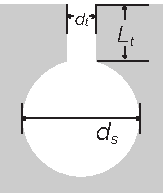
\includegraphics[height=1.25in]{figures/helmholtz_illustration}
            \quad
            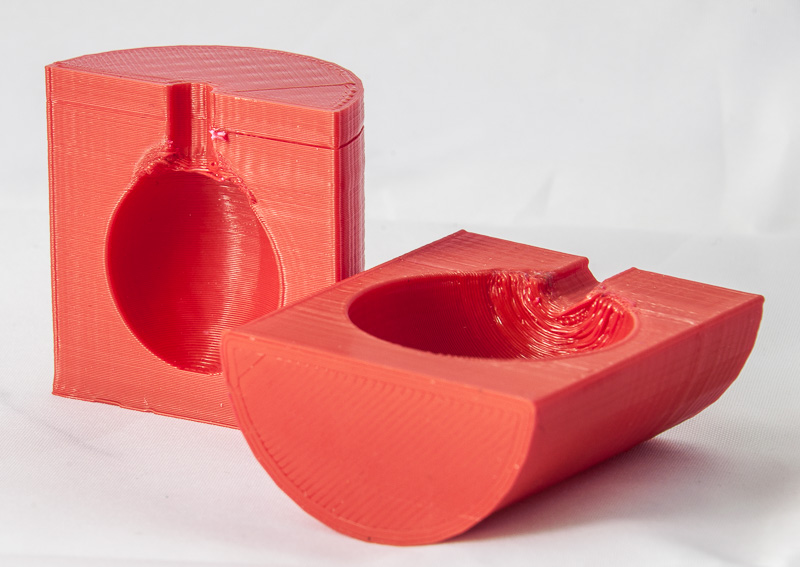
\includegraphics[height=1.25in]{figures/cavities2}
            \caption{Left: an ideal spherical \hhz resonator, with tube
              diameter $d_t$, tube length $L_t$, and sphere diameter $d_s$.
              Right: cross-sections of two \bh test objects, showing the
              resonator structures.}
            \label{fig:resonator}
        \end{figure}

        To better understand the limitations of the frequencies we could detect
        and differentiate between, we took an experimental approach by printing
        48 spherical objects containing different sized cavities inside them (a
        subset of these objects is presented in \cref{fig:cylinders}).  These
        objects were replicated in multiple FDM\footnote{Fused Deposition
        Modeling---the most-common consumer printer technology} printers (Qidi
        Technology X-One, LulzBot Taz 4, and LulzBot Taz Mini) to compare the
        differences in the resulting frequency, if any. We then asked 10 people
        to blow on each cylinder, while we recorded the data using a laptop
        computers' built-in microphone.  \cref{fig:spectrogram} presents
        spectrograms from one for a series of blows into different cavity
        configurations.

        \textbf{Implementation}\\
          As a system, \bh is comprised of three main parts: a design software
          to modify existing 3D models; the objects augmented with resonant
          cavities; and a software that recognizes the sound caused by the user
          blowing into an augmented object, triggering the corresponding
          action.

          \textit{Design Software}\\
            Our software is built on top of Autodesk Meshmixer, making use of
            its Python API to remote control the software, and execute
            commands.  After the user has tagged all the desired positions in
            the model using our software, the user then links them to their
            corresponding actions. \bh then finds a set of $L_t$ and $d_s$ that
            can fit in the requested locations without cavities colliding,
            using a depth-first search algorithm with backtracking. See our
            paper for a detailed explanation of our algorithm.

          \textit{\bh-enabled Objects}\\
            Because our system embeds resonant cavities in existing models, the
            printability of said model is not affected. Thanks to the
            capabilities of most hobbyist 3D-printers to print up to a 45°
            overhang without the need of support material, embedding \bh
            cavities does not cause any extra cleanup on the augmented object
            (aside from removing some ``3D-printer spaghetti'', some can be
            seen in \cref{fig:resonator}). The little to no cleanup and the
            complete lack of assembly required to interact with a \bh-enabled
            object means that the maker can interact with his fabricated object
            directly off the printer.

            \bh-enabled objects can be used for a different number of
            applications. In our paper we present six different uses for
            \bh-enabled objects that illustrates the potential for \bh, from
            those, we present three:

            \underline{Music Controller.} We built a ``music box'' comprised of
              raised controls, each augmented with a \bh cavity inside, capable
              of controlling the music playback by blowing. \bh is robust enough
              to background noise that its performance was not affected by music
              playing in the background.

            \underline{Cell Model.} We augmented a model of an animal
              cell\footnote{\url{http://www.thingiverse.com/thing:689381}} by
              adding \bh tags to different parts of the cell. When the user acts
              on the tags, \bh launches the accompanying Wikipedia cell for the
              corresponding cell component.

            \underline{Interactive Animals.} We fabricated three different
              cetaceous: a
              dolphin\footnote{\url{http://www.thingiverse.com/thing:1121803}},
              and two
              whales\footnote{\url{http://www.thingiverse.com/thing:232247}\\
              \url{http://www.thingiverse.com/thing:665571}}, and set the
              position of the cavity to the animal's blowhole. When these objects
              are interacted with, a corresponding video is played on the user's
              computer.

            \begin{figure}
              \centering
              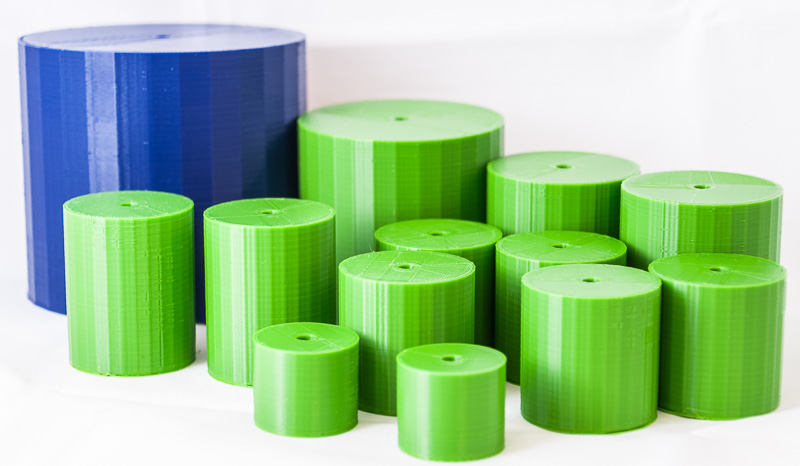
\includegraphics[width=.95\columnwidth]{figures/cylinders.jpg}
              \caption{A subset of our test cylinders with varying cavity
                volumes and tube lengths.}
              \label{fig:cylinders}
            \end{figure}

          \textit{Blow Sound Recognition}\\
            While exploring new wearable interactions in
            Bitey~\cite{Ashbrook:2016ek}, we learned very useful concepts on
            acoustic signal processing and machine learning. We employ these
            concepts in the recognition of the sounds produced when the user
            blows into the \bh cavities. We window the 44.1 KHz signal in 0.1
            second, non-overlapping segments. After computing the RMS value for
            each segment, we look for 0.5 seconds of contiguous windows that
            exceed an empirically set threshold, representing the presence of
            sound. Using Welch's method~\cite{Welch:1967jw}, we extract the
            power spectrum of the signal and use the strongest frequency as the
            resonant frequency of the sound. We then match this frequency to
            the frequencies generated by the set of cavities configurations
            ($d_s$ and $L_t$) to determine which hole the user is interacting
            with. Once classified, we execute the associated action present in
            the configuration file created by the design software.

            The robustness of this algorithm was evaluated against the data
            gathered from our participants, obtaining a 98\% average accuracy
            (please refer to the paper for a complete discussion of these
            results).

        \begin{figure*}[t]
          \centering
            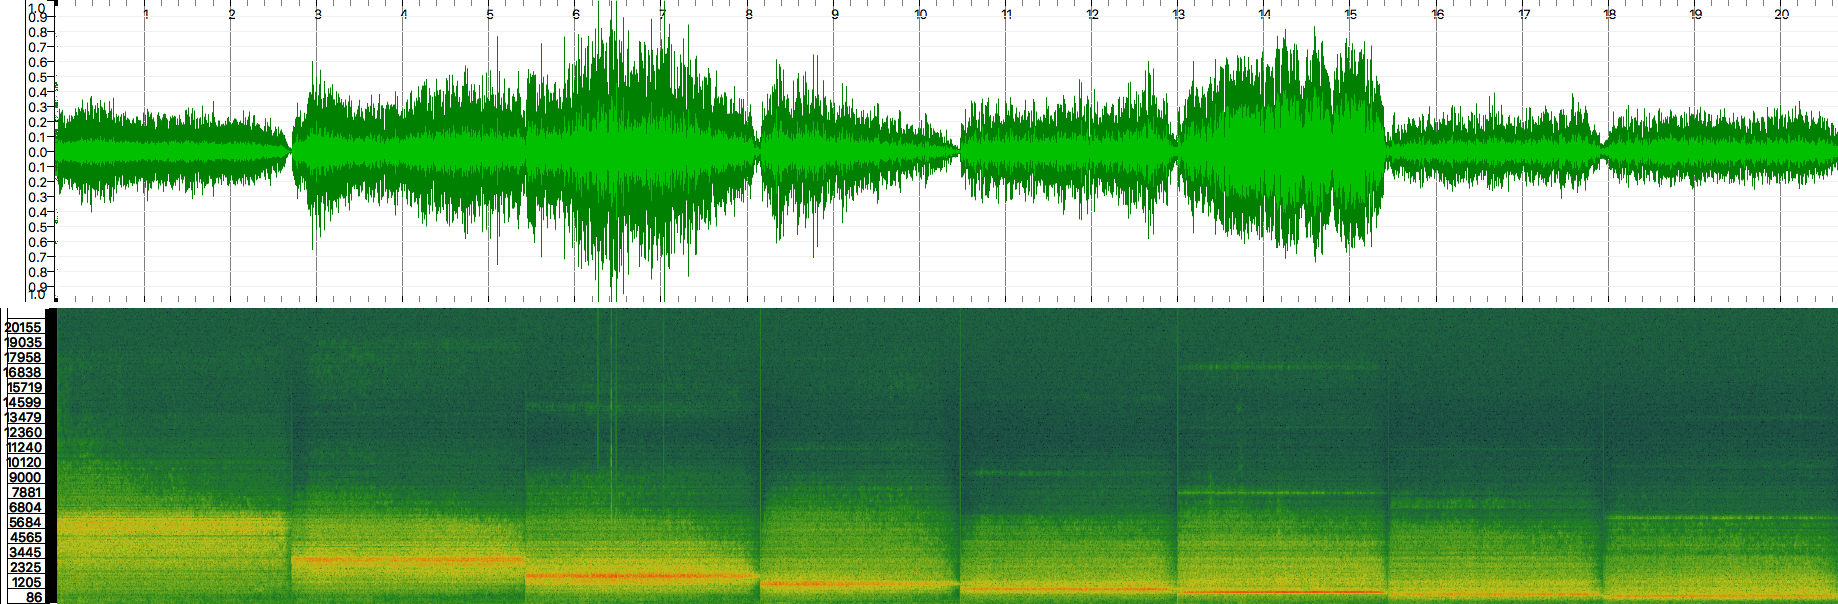
\includegraphics[width=\textwidth]{figures/spectrogram.png}
            \caption{Waveform (top) and spectrogram (bottom) of blows into
              holes with a tube length $L_t$ of 2.5~mm, with the cavity diameter
              $d_s$ varying in steps of 2~mm from 4~mm on the left to 18~mm on
              the right.}
            \label{fig:spectrogram}
        \end{figure*}

      \textbf{Future Work}\\
        We believe that some of the main strengths of \bh is its playfulness
        and its capabilities to translate a physical location on an object to
        an acoustic signature. Therefore, we are interested in exploring how
        \bh is used by children and persons with sight disabilities users in a
        controlled user study. This study will help assess the experience of
        these two populations while using \bh.

    \subsection{New Interaction Mechanisms}
      We continue to explore the different mechanisms we can utilize to enable
      interactivity in 3D-printed models in an maker-friendly way. As we did
      with \bh, we aim to leverage naturally occurring properties to enable
      interactivity in fabricated objects. In this section we will present our
      current, and future, efforts in adding interactivity to 3D-printed
      models.

      \subsubsection{\at}
        For the next addition to our \itoolkit, we draw inspiration from \bh,
        as we continue to leverage sound generated by air currents to enable
        interactivity in 3D-printed objects. We focus our efforts, this time,
        to augment the fabricated objects by adding touch interactivity. As all
        future additions to our toolkit, \at must satisfy the aforementioned
        qualities to guarantee maker-friendliness.

        \begin{figure}
          \centering
            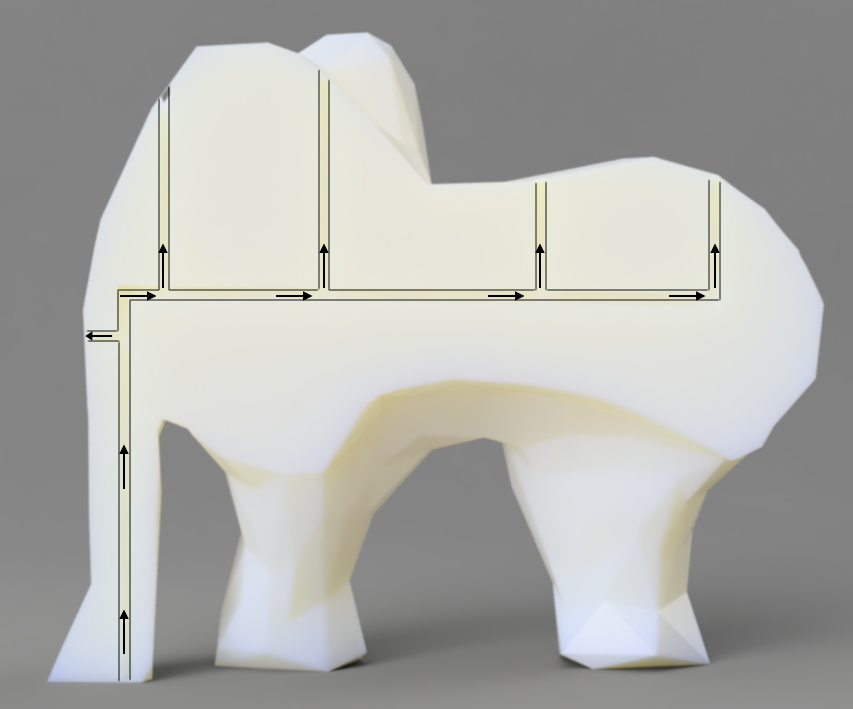
\includegraphics[width=.9\columnwidth]{figures/elephant-airtouch.png}
            \caption{A simplified example of the pipe structure inside a
              3D-printed elephant.}
            \label{fig:elephant-airtouch}
        \end{figure}

        To enable touch interactivity in 3D-printed objects, we will make use
        of Bernoulli's principle for fluid dynamics~\cite{Bernoulli:1738ut} to
        design a system of pipes with openings to the surface, which will be
        embedded inside the fabricated object. When connected to an air source
        (e.g. air compressor), this structure will route the airflow through
        the object to the different places of interest identified by the maker.
        These ducts will be configured in a way that they afford air to flow to
        these openings, but when the opening is covered (e.g. by a finger) the
        air corresponding to that opening is then rerouted through an exhaust
        pipe. Each corresponding exhaust pipe will be corrugated with a unique
        pattern that translates the flow of air into predictable, identifiable,
        sounds, in a similar fashion how He \etal explore in
        SqueezaPulse~\cite{He:2017jc}. \cref{fig:elephant-airtouch} presents a
        simplified model of how these air ducts will look inside a 3D-printed
        elephant, where the airflow begins in the elephant's trunk and is then
        propagated using the previously described structure.

        These structures can enable a variety of touch interactions on the
        3D-printed object, ranging from simple touch interactions, to more
        complex gestures like sliding and long-presses. We will enable these
        interactions by analyzing the duration of the already identified
        signal.

        Similarly to \bh, \at will be made up of three main components: a
        design system that allows users to modify existing three dimensional
        models, the \at-enabled objects, and a wearable-based recognition
        software that identifies the emitted sound, triggering the
        corresponding action.

        Once we finish developing \at, our next step will be to evaluate the
        usability of our system. To do so, we will recruit up to 15 novice
        makers from the local makerspace and carry out a user study. In the
        study, we will observe how the participants use \at to augment existing
        designs with touch interactivity. We will proceed to note their
        experiences while modifying, fabricating and interacting with the
        fabricated object. These results, alongside with the results from \bh,
        will shape our future endeavors in this space.

  \section{Conclusion}
    In this paper we presented and analyzed the obstacles that plague the
    current state-of-the-art in the fabrication of interactive objects. In
    response to the aforementioned limitations, we introduce  our effort to
    lower the complexity on adding interactivity to fabricated objects by
    leveraging natural properties. Our solution takes the form of an \itoolkit
    where the maker can choose which mechanisms to augment its object with. As
    a first addition to this toolkit, we introduced Blowhole, a system that
    allows the maker to tag three dimensional models using blowing-activated
    tags. Additionally, we present our current efforts in populating our
    \itoolkit with \at. Here, we will embed a system of air ducts inside a
    three dimensional model to leverage touch interactions and enable a variety
    of gestures.

  \bibliographystyle{SIGCHI-Reference-Format}
  \bibliography{papers}

  \newpage
  \section{Appendix}
    This work was performed in the Future Everyday Technology Research
    Laboratory (FETLab) under the supervision of Dr. Daniel Ashbrook, the
    director of this space. The FETLab focuses its work in the democratization
    of digital fabrication technologies (e.g. 3D printing, laser cutting, CNC
    milling). The premise behind their work is that, although digital
    fabrication equipment are now reasonably priced to be afforded by
    enthusiasts and hobbyists, the tools and process accompanying these still
    present high levels of difficulty which not all novices can reach. The work
    presented on \bh was carried out by the Acoustic Interfaces group comprised
    of Zhiyuan Li, Osamu Fujimoto, and myself, where Zhiyuan was responsible
    for the implementation of the design software, Osamu focused on
    experimenting with the different cavity shapes and sizes, and I was
    responsible of the development of the sound recognition section.

\end{document}
